\subsection{Supporting Technologies}
\label{sec:supportingTechnologies}

Revisiting the rapport model described throughout Chapter~\ref{chap:rapportModel}, the rapport \textit{Effectors} require the following perceptual capabilities:
\begin{itemize}
	\item Monitor the interaction activity, for the Positivity \textit{Effectors}.
	\item Identify human emotions, and head-gestures for the behavioural mimicry \textit{Effectors};
	\item Identify speech disfluencies (Figures~\ref{fig:lowering} to \ref{fig:risingLowering}) for the backchannel \textit{Effector};
	\item Identify the user's gender and monitor the current state of the interaction, for the Mutual-Gaze \textit{Effector};
\end{itemize}

Following Figure~\ref{fig:SupportingTechnologiesOverview}, the system uses \ac{SSI}~\footnote{\url{http://hcm-lab.de/projects/ssi/}} to recognise social-signals in real-time from microphones and video feeds~\cite{Wagner2013}. \ac{SSI} uses SHORE~\cite{Ruf2011} and openSMILE~\cite{Eyben:2013:RDO:2502081.2502224} to recognise emotions, and extract prosody features, respectively. For example, \ac{SSI} identifies head-gestures using a Kinect Camera, and SHORE outputs the different emotion intensities given the video feed. Finally, \ac{SSI} periodically collects and sends the perceptual information in \ac{XML} format through network messages to other processes using ActiveMQ~\footnote{\url{http://activemq.apache.org/}}, specifically GRETA\textsuperscript{PP}.

\begin{figure}[H]
	\centering
	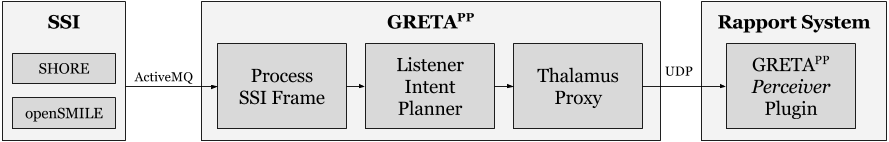
\includegraphics[width=0.95\textwidth]{images/SupportingTechnologiesOverview.png}
	\caption{Schematic representation of the components that supports the rapport model.}
	\label{fig:SupportingTechnologiesOverview}
\end{figure}

GRETA\textsuperscript{PP} is a variation of the GRETA system~\cite{Niewiadomski2009} that uses only the  \textit{Listener Intention Planner} component of the original GRETA (Figure~\ref{fig:GretaOriginal}), as we are not interested in the remaining components for the scope of this thesis. In short, GRETA\textsuperscript{PP} attempts to match the perceptual information to the first behavioural rule defined in a configuration file loaded at launch as exampled in Listing~\ref{lst:exampleGretaRule}. In the case of a match, the system might output a response signal given the response probability specified by the same rule. The original set of rules was reduced, as they were tailored for a virtual agent with different capabilities than the robot \ac{EMYS}, for example, the virtual agent is capable of moving his eyebrows and specific lip positions. Finally, taking advantage that GRETA is already integrated with \ac{SSI}, we adapted \ac{SSI} and GRETA\textsuperscript{PP} to redirect head gestures and facial expressions perceptual information to our system. It is important to mention that there is a slight delay beginning from \ac{SSI} and ending in the \textit{Perceiver}, and that only the emotion with the highest intensity is sent. The major bottleneck of the system relies on \ac{SSI} itself which is resource intensive and, in order to be able to test the system, the refresh rate had to be reduced to 5Hz which is half the default value.


\begin{lstlisting}[caption={One of the backchannels rules used GRETA and GRETA\textsuperscript{PP}.},label={lst:exampleGretaRule},language=XML]
<rule name="trigger-rise-fall">
	<usersignals>
		<usersignal id="1" name="rise_fall" modality="speech"/>
	</usersignals>
	<backchannels probability="1.0" priority="2">
		<response_reactive probability="0.4"/>
	</backchannels>
</rule>
\end{lstlisting}

Lastly, the communication with the rapport system is accomplished using \ac{UDP} sockets to transmit information in real-time without concerning with packet-loss as the system runs locally. The GRETA\textsuperscript{PP} \textit{Perceiver} Plugin, given the perceptual information, will notify the interested \textit{Effectors}.

\begin{figure}[H]
	\centering
	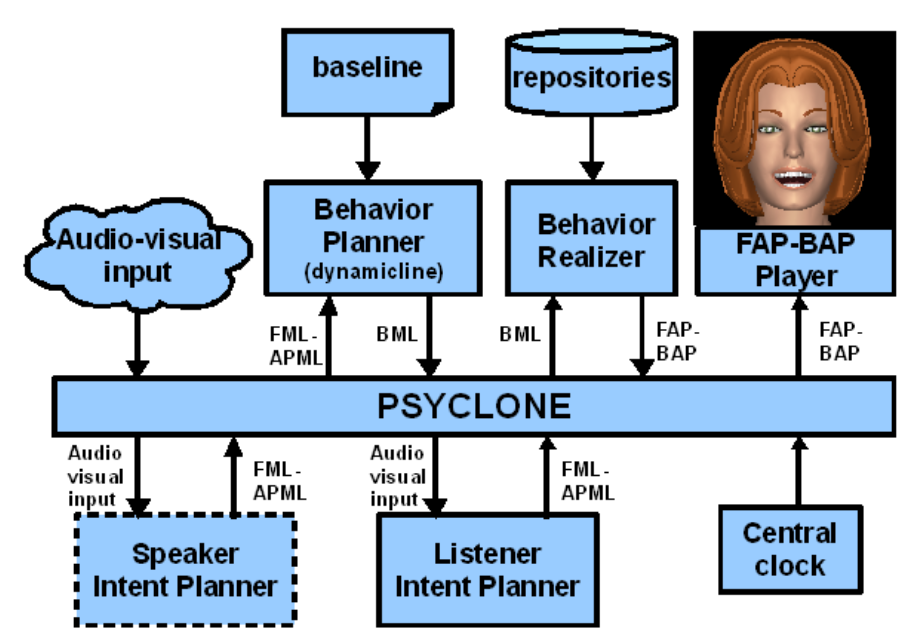
\includegraphics[width=0.6\textwidth]{images/GretaArchitecture.png}
	\caption{GRETA architecture. From~\cite{Niewiadomski2009}}
	\label{fig:GretaOriginal}
\end{figure}



% there are four main modules  that supports the rapport strategies:
%\begin{itemize}
%	\item \textbf{\ac{SSI}}: recognise social signals in realtime;
%	\item \textbf{SHORE}: recognise emotions from a video feed;
%	\item \textbf{GRETA\textsuperscript{PP}}: adapted version of GRETA~\cite{Niewiadomski2009} to generate listener behaviour;
%	\item \textbf{GRETA \textit{Perceiver} Plugin}: proxy between GRETA\textsuperscript{PP} and the \textit{Rapport Controller}.
%\end{itemize}

